\documentclass{article}
\usepackage[utf8]{inputenc}
\usepackage[english]{babel}
\usepackage[T1]{fontenc}
\usepackage{csquotes}
\usepackage{graphicx}
\usepackage{listings}
\usepackage{listingsutf8}
\usepackage{listingsutf8}
\usepackage{listingsutf8}
\usepackage{listingsutf8}
\usepackage{listingsutf8}
\usepackage{listingsutf8}
\usepackage{listingsutf8}
\usepackage{listingsutf8}
\usepackage{listingsutf8}
\usepackage{listingsutf8}
\usepackage{listingsutf8}
\usepackage{listingsutf8}
\usepackage{listingsutf8}
\lstset{
basicstyle=\ttfamily\footnotesize,
language=Python,
columns=fullflexible,
breaklines=true
}
\usepackage{hyperref}

\begin{document}

\title{Implementation of Drawing Recognition Model (CAD2Program) in JAX/Flax}
\author{}
\date{}
\maketitle

\section{Model Architecture Overview}

The model is based on the CAD2Program approach, which proposes converting drawings into text programs describing geometry. The architecture has two main components: a Vision Transformer (ViT) for encoding drawing images and a transformer decoder for generating text sequences describing geometric primitives and their parameters. This approach belongs to the category of vision-language models that combine vision and language, similar to multimodal models (e.g., GPT-4V, LLaVA, etc.).

\paragraph{ViT Image Encoder.} The input drawing (scan or photo of a hand-drawn drawing) is processed by a ViT encoder, which splits the image into patches (e.g., $16\times16$ pixels) and converts them into a sequence of embeddings of fixed dimensionality. A learnable class token and positional embeddings are added to the sequence of patches, after which it is passed through several transformer encoder layers. ViT extracts high-level features from the image; in particular, the class token (or averaged representation of patches) serves as an integral representation of the entire drawing. ViT models have proven to be effective image encoders in various computer vision tasks, and in this case allow processing the drawing as a whole as a raster image, without requiring preliminary extraction of vector elements or layer separation.

\paragraph{Transformer Decoder (Language Model).} The output of the ViT encoder goes to a transformer decoder, whose task is to generate a sequence of tokens describing geometric primitives and their parameters. In the CAD2Program work, a large language model (LLM) InternLM-1.8B is used as the decoder, which receives a text prompt as input and additionally multimodal image embeddings. In our implementation, we can use a similar principle: the decoder autoregressively predicts text token by token, at each step taking into account previously generated tokens (self-attention) and image features from the encoder (cross-attention). Thus, the model generates a description of the drawing in the form of a \textit{program}: a list of primitives (rectangles, circles, arcs, polylines, etc.) and corresponding parameters (coordinates, dimensions, angles, radii, etc.).

It is important to emphasize that the model's output is presented in text form, which provides several advantages. First, text descriptions can be easily extended with new types of primitives or properties without changing the model structure. Second, using text, the model can output numerical parameter values with virtually no loss of accuracy, avoiding quantization errors – numbers are simply copied from drawing annotations (e.g., dimension lines) to the response. Third, the language model has knowledge of syntax and can generate output in pseudo-code format or ready-to-execute scripts (e.g., in Python, as in CAD2Program). This vision-language approach allows the model to simultaneously analyze visual elements of the drawing (geometry and text annotations) and form semantically rich descriptions in human-readable form.

\begin{figure}[h!]
\centering
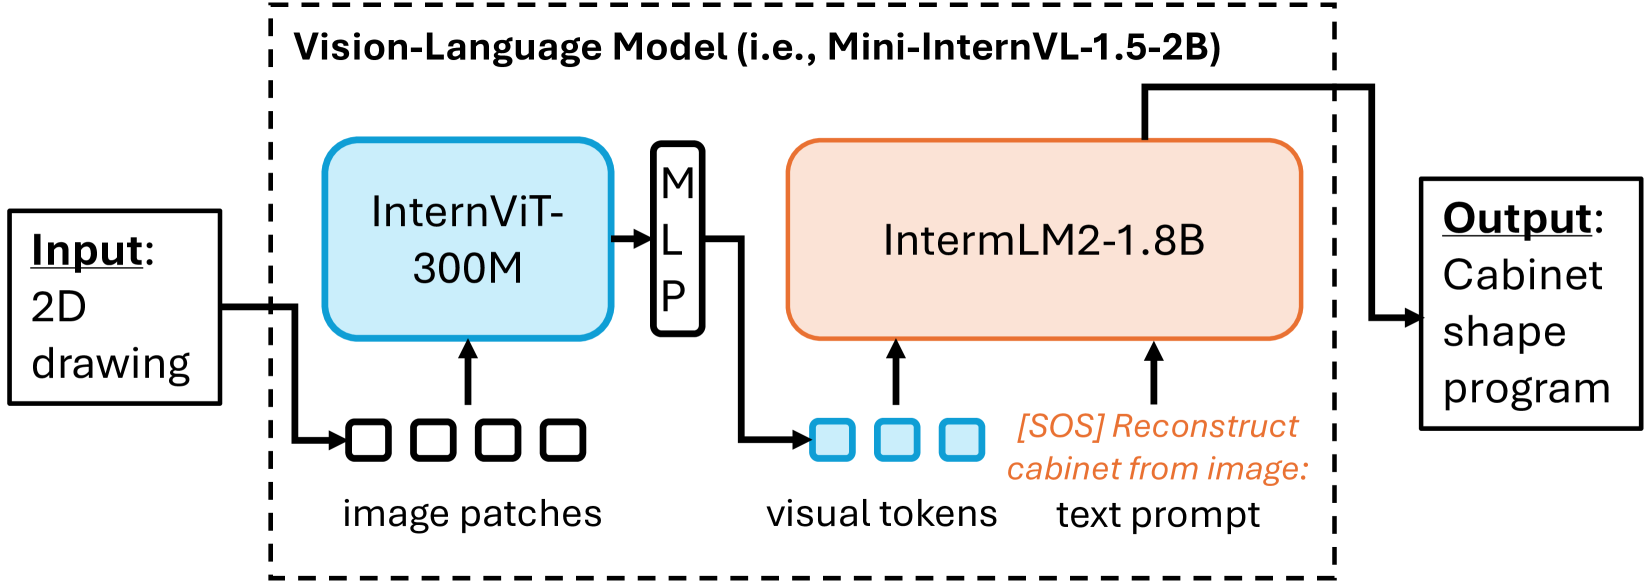
\includegraphics[width=0.95\textwidth]{internvl.png}
\caption{Overview of CAD2Program model architecture: ViT encoder (InternViT) extracts features from the drawing image, MLP projection maps them to the decoder's hidden space, and the language model (InternLM) generates a text program of primitives.}
\end{figure}

\textbf{Figure 1} shows a diagram of such an architecture corresponding to the CAD2Program model. For multimodal integration, a small fully connected projector (MLP) is used, which converts the encoder output into a format suitable for input to the language model. In the original CAD2Program, a text prompt "\texttt{Reconstruct cabinet from image:}" was fed to the decoder before the main output, but in our case we can use a simpler prompt (or a special sequence start token). During generation, the decoder combines visual context (image embeddings) and the history of generated tokens, sequentially producing a list of primitives with parameters.

The vision-language approach is justified by the fact that a 2D drawing contains both geometric and textual information (dimensions, labels). Previously, many 3D reconstruction methods ignored annotations and worked only with geometry, requiring preliminary separation of text. Our model, however, learns to directly "read" the drawing in all its diversity, extracting dimensions and other marks from the image. This became possible thanks to the use of a large pre-trained language model capable of understanding text and numbers, as well as training on a large dataset including diverse drawings with their descriptions. As a result, the model achieves accuracy comparable to methods working with vector CAD input, although it operates only on raster images.

\section{Step-by-Step Model Implementation in JAX/Flax}

Below is an implementation of the described model using JAX/Flax. We will consider data preparation, creating the encoder and decoder architecture, the model training process, and performing inference on new images. The code will be provided in Python using the Flax library (which implements the main neural network components for JAX).

\subsection{Data Preparation}

To train the model, a set of {\textit{drawing, program-description}} pairs is needed. Ideally, one can collect a real dataset of technical drawings with annotations. If such is not available, synthetic data generators are used. For example, \textbf{Free2CAD} generates random object sketches and corresponding CAD command scripts for them. Similarly, one can automatically create images of primitives with dimension lines: randomly place rectangles, circles and other shapes, add text labels (lengths, radii) to them, then render the resulting drawing into an image. At the same time, a target text sequence is generated: a list of primitives and their parameters that match the image.

When real data is available (e.g., drawing scans), preliminary annotation may be needed: manually or semi-automatically describe each drawing with a set of primitives. However, the CAD2Program approach assumes that the model will learn to extract primitives and read their dimensions itself, so an explicit annotator may not be needed – it is sufficient to have ready correspondences between images and parameters from which a program text can be formed.

Drawing images are converted to tensors (e.g., numpy or JAX arrays) of fixed size. Usually, scaling (e.g., $224\times224$ pixels) and pixel value normalization are applied. Text descriptions (programs) are tokenized – split into tokens according to the vocabulary. One can use either a ready-made language model tokenizer (if the decoder is based on a pre-trained LLM) or a specialized tokenizer that takes into account the description format (e.g., separating primitive names and numbers). In the simplest case, each character can be considered a separate token, but it is more efficient to apply byte-pair encoding or SentencePiece for encoding parameter strings. At the output of data preparation, we get a set of training examples of the form:
$$X_i = \text{image}_i,\qquad Y_i = [t_1, t_2, \dots, t_{N_i}],$$
where $Y_i$ is the sequence of target tokens for drawing $i$.

For subsequent use in JAX, data is often packaged into \texttt{tf.data.Dataset} or TFRecord format, but one can also work with regular numpy arrays, splitting them into batches. The main thing is to organize efficient reading and augmentations (e.g., random rotations or adding noise to images to increase model robustness to handwritten variations).

\subsection{Model Architecture in Flax}

We define two main Flax modules: \texttt{VisionEncoder} for the ViT encoder and \texttt{TextDecoder} for the autoregressive decoder. Below is simplified code implementing these modules.

\begin{lstlisting}
import jax.numpy as jnp
from flax import linen as nn

# Vision Transformer Encoder

class VisionEncoder(nn.Module):
    embed_dim: int = 768
    patch_size: int = 16
    num_layers: int = 12
    num_heads: int = 12

    def setup(self):
        # Patch projection and class token
        self.patch_embed = nn.Dense(self.embed_dim)
        self.cls_token = self.param('cls_token', nn.initializers.normal(stddev=0.02), (1, 1, self.embed_dim))
        self.pos_embedding = self.param('pos_embedding', nn.initializers.normal(stddev=0.02),
                                        (1, (image_size//self.patch_size)**2 + 1, self.embed_dim))
        # Transformer Encoder layers
        self.transformer_layers = [nn.SelfAttention(num_heads=self.num_heads) for _ in range(self.num_layers)]
        self.mlp_layers = [nn.Sequential([
                                  nn.Dense(self.embed_dim*4), nn.gelu, nn.Dense(self.embed_dim)
                              ]) for _ in range(self.num_layers)]
        self.norm = nn.LayerNorm()

    def __call__(self, img):
        # img shape: (H, W, 3)
        patches = extract_patches(img, patch_size=self.patch_size)  # user-defined function
        tokens = self.patch_embed(patches)  # shape: (num_patches, embed_dim)
        # prepend CLS token
        cls = jnp.tile(self.cls_token, (tokens.shape[0], 1, 1))    # (batch, 1, embed_dim)
        x = jnp.concatenate([cls, tokens], axis=1) + self.pos_embedding  # add positional embeddings
        # Transformer encoder
        for sa, mlp in zip(self.transformer_layers, self.mlp_layers):
            # Multi-head self-attention block
            x = x + sa(x)              # residual connection
            x = x + mlp(x)            # MLP block with residual
        encoded = self.norm(x)        # shape: (batch, 1+num_patches, embed_dim)
        return encoded
\end{lstlisting}

In the encoder code above, we omitted the details of the \texttt{extract_patches} function, which splits the image into patches and arranges them in a sequence (dimension \texttt{num_patches} = $(H/\texttt{patch_size})\times(W/\texttt{patch_size})$). After projecting patches with a linear layer and adding a learnable \texttt{[CLS]} token, $L$ transformer layers are executed: each layer includes multi-head self-attention and a subsequent MLP (fully connected layer with GELU activation and output projection), both with residual connections and normalization layer (LayerNorm). The output \texttt{encoded} has dimension $(B, N_p+1, D)$, where $B$ is the batch size, $N_p$ is the number of patches, $D$ is the embedding dimension. For transmission to the decoder, either the entire set of patch embeddings or only the class token embedding (as a generalized representation of the image) is usually used. In CAD2Program, for example, the entire set of visual tokens (split into image tiles) was used.

Now let's define the decoder. In a simplified version, this is an autoregressive transformer that at each step generates the next token, having access to previous tokens (through self-attention) and to the encoded image (through cross-attention). We can use a standard transformer decoder from Flax, but for demonstration we'll write the scheme manually:

\begin{lstlisting}
# Transformer Decoder with cross-attention

class TextDecoder(nn.Module):
    vocab_size: int
    embed_dim: int = 768
    num_layers: int = 12
    num_heads: int = 12

    def setup(self):
        # Token embedding and positional embedding
        self.token_embed = nn.Embed(self.vocab_size, self.embed_dim)
        self.pos_embedding = self.param('dec_pos_embedding', nn.initializers.normal(stddev=0.02),
                                        (1, max_seq_len, self.embed_dim))
        # Transformer Decoder layers
        self.self_attn_layers = [nn.SelfAttention(num_heads=self.num_heads) for _ in range(self.num_layers)]
        self.cross_attn_layers = [nn.MultiHeadDotProductAttention(num_heads=self.num_heads) for _ in range(self.num_layers)]
        self.mlp_layers = [nn.Sequential([
                                  nn.Dense(self.embed_dim*4), nn.gelu, nn.Dense(self.embed_dim)
                              ]) for _ in range(self.num_layers)]
        self.norm = nn.LayerNorm()
        # Final language modeling head
        self.output_proj = nn.Dense(self.vocab_size)

    def __call__(self, encoded_image, input_tokens):
        # encoded_image: (batch, N_enc, D), input_tokens: (batch, T)
        x = self.token_embed(input_tokens) + self.pos_embedding[:, :input_tokens.shape[1], :]
        # Masked self-attention to prevent looking ahead
        attn_mask = nn.make_causal_mask(input_tokens)  # triangle causal mask
        for sa, ca, mlp in zip(self.self_attn_layers, self.cross_attn_layers, self.mlp_layers):
            x = x + sa(x, mask=attn_mask)              # self-attention (causal)
            x = x + ca(query=x, key=encoded_image, value=encoded_image)  # cross-attention
            x = x + mlp(x) 
        x = self.norm(x)
        logits = self.output_proj(x)  # shape: (batch, T, vocab_size)
        return logits
\end{lstlisting}

Here \texttt{nn.MultiHeadDotProductAttention} is a Flax module that implements the "query-key-value" attention mechanism between two sequences (i.e., used for cross-attention with keys/values from the encoder and queries from the decoder). We use a causal mask (\texttt{make_causal_mask}) for self-attention so that the decoder cannot see future tokens in the sequence. At the decoder output, we get \textit{logits} of dimension $(B, T, V)$, where $T$ is the sequence length, $V$ is the vocabulary size. To obtain probabilities, softmax is applied along dimension $V$. During training, we will compare these logits with the true sequence of tokens.

Finally, let's combine the encoder and decoder into one model for training convenience:

\begin{lstlisting}
class CADModel(nn.Module):
    vocab_size: int
    # Encoder/decoder parameters omitted for brevity
    
    def setup(self):
        self.encoder = VisionEncoder()
        self.decoder = TextDecoder(vocab_size=self.vocab_size)
    
    def call(self, image, input_tokens):
        enc = self.encoder(image)  # (B, N_enc, D)
        logits = self.decoder(encoded_image=enc, input_tokens=input_tokens)
        return logits
\end{lstlisting}

Note that for autoregressive training, the decoder receives in \texttt{input_tokens} the correct sequence shifted by one step (Teacher Forcing): for example, \texttt{input_tokens} = $[\langle \text{BOS}\rangle, t_1, t_2, \dots, t_{N-1}]$, and target tokens for loss calculation = $[t_1, t_2, \dots, t_{N-1}, t_N, \langle \text{EOS}\rangle]$. Thus, at the $i$-th step, the decoder sees all previous correct tokens and learns to predict the next $t_i$.

When initializing the model, pre-trained weights can be used: for example, initialize \texttt{VisionEncoder} from a ViT model trained on ImageNet, and \texttt{TextDecoder} from a pre-trained language model (with appropriate loading of embeddings and transformer layers). In the case of CAD2Program, ready-made weights from InternViT and InternLM were used, which significantly accelerated training and improved quality. In our implementation, for simplicity, we can start training "from scratch" or load a model with similar architecture (e.g., ViT-B/16 and some GPT-2/T5 for the decoder) and then fine-tune it on our task.

\subsection{Model Training}

Training is conducted by minimizing the cross-entropy loss function between predicted and true program tokens. After each decoder step, we have a distribution $\hat{y}_i$ over the vocabulary, and compute $-\sum_i y_{i}\log \hat{y}_i$, where $y_i$ is the one-hot representation of the correct token at this step. The loss is averaged over all tokens in the sequence and over the batch:
$$L(\theta) = - \frac{1}{B}\frac{1}{T}\sum_{b=1}^B \sum_{t=1}^{T} \log P_\theta(y_{b,t} \mid x_b, y_{b,<t}),$$
where $x_b$ is the image, $y_{b,<t}$ are the already generated tokens up to step $t$ (teacher forcing ensures that these are real tokens during training).

In JAX for training, we compile the loss function and its gradient. We use Optax (optimizer library for JAX) to define the optimizer, for example AdamW. Below is a sketch of the training loop:

\begin{lstlisting}
import optax
from flax.training import train_state

# Create model object and initial parameter state

model = CADModel(vocab_size=len(vocab))
rng = jax.random.PRNGKey(0)
params = model.init(rng, jnp.zeros((1, image_size, image_size, 3)),
                    jnp.zeros((1, max_len), dtype=jnp.int32))['params']

# Define training state

tx = optax.adamw(learning_rate=1e-4)
state = train_state.TrainState.create(apply_fn=model.apply, params=params, tx=tx)

@jax.jit
def train_step(state, batch):
    """Performs a training step on one batch of data."""
    def loss_fn(params):
        logits = model.apply({'params': params}, batch['image'], batch['input_tokens'])
        # compute cross-entropy loss
        labels = batch['target_tokens']  # expected tokens (shape: [B, T])
        loss = optax.softmax_cross_entropy_with_integer_labels(logits, labels).mean()
        return loss
    # compute loss function value and gradients
    loss, grads = jax.value_and_grad(loss_fn)(state.params)
    # update parameters
    new_state = state.apply_gradients(grads=grads)
    return new_state, loss

# Iterative training

for epoch in range(num_epochs):
    for batch in data_loader:
        state, loss = train_step(state, batch)
        print(f"Epoch {epoch}: loss = {loss}")
\end{lstlisting}

In this code, \texttt{train_state} is a convenient wrapper from Flax that stores parameters and the optimizer. The \texttt{train_step} function is marked with \texttt{@jax.jit} for compilation and execution on GPU/TPU, which significantly speeds up training. Inside, we compute gradients of the loss function using \texttt{jax.value_and_grad}. \texttt{optax.softmax_cross_entropy_with_integer_labels} is used, which takes logits and target token indices, returning a loss vector for each element, after which we take the mean. Gradients are applied through \texttt{state.apply_gradients}, which internally performs an optimizer step (AdamW).

It should be noted that training a full model from scratch is a resource-intensive process. In the original CAD2Program work, training was conducted on 64 GPUs (RTX 4090) for about a day on a dataset of $\sim$368k drawings. In our conditions, the volumes may be smaller, but still dozens of epochs on large batches may be required for convergence. Pre-training the encoder/decoder reduces the necessary training time.

\subsection{Inference (Description Generation)}

After training (or during validation), it is necessary to implement inference: obtaining a sequence of primitives from an input image. Here the model works in autoregressive generation mode. One can use standard text generation methods applied to language models – for example, greedy search (greedy decoding) or beam search. For simplicity, we'll describe the greedy approach:
\begin{enumerate}
\item Get image embeddings through the encoder: $h = \text{encoder}(image)$.
\item Initialize the output sequence with a start token (e.g., \texttt{<BOS>} or just empty context).
\item Pass the current token sequence to the decoder and get logits for the next token.
\item Select the token with maximum probability (argmax over logits of the last step) and add it to the sequence.
\item If the token turns out to be an end-of-sequence token (\texttt{<EOS>}) or the maximum allowed length is reached, stop generation. Otherwise, return to step 3.
\end{enumerate}

Below is pseudocode (in Python) for the generation function:

\begin{lstlisting}
def generate_primitives(params, image, max_len=100):
    enc = model.encoder.apply({'params': params['encoder']}, image)
    tokens = [vocab['<BOS>']]
    for t in range(max_len):
        logits = model.decoder.apply({'params': params['decoder']}, enc, jnp.array([tokens], dtype=jnp.int32))
        next_token = int(jnp.argmax(logits[0, -1]))
        if next_token == vocab['<EOS>']:
            break
        tokens.append(next_token)
    return [vocab.id_to_token[t] for t in tokens[1:]]
\end{lstlisting}

This function (assuming that \texttt{params} is divided into sub-dictionaries for encoder and decoder) returns a list of generated tokens (without the initial BOS). From these tokens, one can then reconstruct the structure of primitives. For example, if the output tokens form a string \texttt{"rectangle(x=10,y=15,w=40,h=20); circle(x=30,y=5,r=5)"}, it needs to be parsed into the necessary parameters or directly interpreted as commands. In CAD2Program, the output was formed as syntactically correct Python code with variable assignments that can be executed to obtain a 3D model. In our case, it's sufficient to get a data structure – a list of dictionaries or objects, for example:
$$[ \{\text{type}: \text{"rectangle"}, x:10, y:15, w:40, h:20\}, \{\text{type}:\text{"circle"}, x:30, y:5, r:5\} ].$$

To improve inference reliability, one can apply beam search (storing several most probable sequences and expanding them) or add temperature sampling, repetition penalty, and other techniques from NLP to greedy selection. However, the task is deterministic based on annotations on the drawing, so greedy search is usually sufficient – the model should unambiguously output the correct numbers and types of primitives.

\section{Integration with ClearML}

For convenience of experiments and tracking metrics, we integrate the training and inference process with the ClearML platform. ClearML provides automatic logging of parameters and results, model storage, and simple deployment through ClearML-Serving. Below are the main integration steps.

\subsection{Experiment and Metrics Logging}

Integration begins with initializing the experiment task in ClearML. In code, this is done with the command:
\begin{lstlisting}
from clearml import Task
task = Task.init(project_name=“CADPrimitives”, task_name=“Train CAD2Program model”)
\end{lstlisting}
After this, the running script connects to the ClearML server (local or cloud). ClearML automatically collects information about the environment, launch parameters, and even the models used.

Hyperparameters (e.g., layer sizes, learning rate, batch size) can be logged through \texttt{task.connect} so they appear in the interface:
\begin{lstlisting}
config = {"embed_dim": 768, "num_layers": 12, "lr": 1e-4, "batch_size": 32}
task.connect(config)
\end{lstlisting}
This will save the experiment parameters dictionary.

During training, we can send metric values to ClearML. ClearML automatically picks up standard metrics from popular frameworks, but in the case of manual training on JAX, it's worth explicitly using \texttt{Logger}:
\begin{lstlisting}
from clearml import Logger
logger = task.get_logger()

for epoch in range(num_epochs):
    for batch in data_loader:
        state, loss = train_step(state, batch)
    # Log error after each epoch
    logger.report_scalar("loss", "train", epoch, float(loss))
\end{lstlisting}
The \texttt{report_scalar} command records a scalar value (e.g., \texttt{loss}=0.024) in the current iteration (epoch). In the ClearML web interface, these points will be displayed on a graph. Similarly, one can log accuracy metrics, step time, or arbitrary data. For example, it's possible to log examples of generated descriptions for the validation set using \texttt{logger.report_text} or add drawing images with overlaid recognized primitives through \texttt{report_image}.

ClearML also saves stdout/stderr of your script, which simplifies debugging. As a result, each training run will be documented: what code and parameters were used, what metrics were obtained, what artifacts were saved. This ensures reproducibility of experiments and convenient comparison of different model runs.

\subsection{Model and Checkpoint Saving}

After (or during) training, it is necessary to save the model weights. Since Flax stores parameters as immutable dictionaries, they can be serialized using \texttt{flax.serialization.to_bytes} or \texttt{pickle}. For example:
\begin{lstlisting}
import os, pickle

# Serialize parameters

weights_bytes = flax.serialization.to_bytes(state.params)
with open("model_ckpt.pkl", "wb") as f:
    f.write(weights_bytes)
\end{lstlisting}
This file \texttt{model_ckpt.pkl} contains the state of the trained model. We can save checkpoints periodically (e.g., every $N$ iterations) for protection against failures and for the ability to rollback to the best version (by metric).

ClearML provides a convenient way to store such models: \textbf{OutputModel}. We can either manually upload the file as an experiment artifact, or use the \texttt{Task.update_output_model} method. One simple way:
\begin{lstlisting}
from clearml import OutputModel
OutputModel.update_checkpoint(task=task,
                              iteration=num_epochs,
                              path="model_ckpt.pkl",
                              name="CAD2Program_model")
\end{lstlisting}
This command will upload the file \texttt{model_ckpt.pkl} to ClearML storage (e.g., to ClearML Server or cloud storage) and assign it a name. After this, the experiment in the interface will correspond to a \emph{model} that can be downloaded or immediately deployed.

Alternatively, one can call \texttt{task.upload_artifact("model_final", "model_ckpt.pkl")}, then the file will be bound as an artifact. The difference is that \texttt{OutputModel} registers specifically the model and its metadata, and it's easier to use later with ClearML-Serving.

\paragraph{Deployment via ClearML-Serving.} After the model is registered, we can deploy it using ClearML-Serving for remote inference. ClearML-Serving consists of a service (controller) and one or more inference worker processes that can be run in Docker containers. Interaction occurs through the CLI \texttt{clearml-serving}. Main deployment steps:
\begin{enumerate}
\item Start Serving service: create a new service task in ClearML (e.g., through web interface or CLI). It will get its identifier (Service ID). For example, let \texttt{service_id = SERV1234}.
\item Model registration in service: execute CLI command on the machine where \texttt{clearml-serving} is installed:
\begin{verbatim}
$ clearml-serving --id SERV1234 model add \
    --engine "python" \
    --endpoint "cad_model" \
    --model-id "<Model ID in repository>" \
    --preprocess "preprocess.py" \
    --postprocess "postprocess.py"
\end{verbatim}
The \texttt{--model-id} parameter points to the unique ID of the model saved in ClearML (it can be copied from the UI, or ClearML will print it when registering the model). \texttt{--engine "python"} means that we ourselves will define how to perform inference (unlike, say, \texttt{--engine torchserve} or \texttt{triton} for standard frameworks). This is a flexible mode where we can set arbitrary Python preprocessing and postprocessing. Files \texttt{preprocess.py} and \texttt{postprocess.py} are scripts that will be executed before sending the request to the model and after receiving the response. In them, we describe how to transform the input image (e.g., read image bytes from HTTP request, convert to tensor of the required shape, possibly perform augmentations) and how to process the model output (e.g., convert list of tokens to convenient JSON with primitives). These scripts will also be packaged by ClearML-Serving and stored on the server.
\item Start inference container: ClearML-Serving allows running inference as a Docker container. For this, it's sufficient to execute:
\begin{verbatim}
$ docker run -d -p 8080:8080 -e CLEARML_SERVING_TASK_ID=SERV1234 \
    -e CLEARML_SERVING_POLL_FREQ=5 clearml-serving-inference:latest
\end{verbatim}
Here we assume that the \texttt{clearml-serving-inference:latest} image is already built (if not, it can be built from the ClearML-Serving repository). The \texttt{CLEARML_SERVING_TASK_ID} variable tells the container which service (with which ID) it serves, and \texttt{POLL_FREQ} – how often to check for updates. After startup, the container will connect to ClearML Server, load the registered model, and be ready to accept requests.
\item Inference call: By default, the container listens on port 8080. ClearML-Serving creates a REST API for each \texttt{endpoint}. We specified \texttt{--endpoint "cad_model"}, so the URL will be \verb|http://localhost:8080/serve/cad_model|. By sending an HTTP POST request to this address with input data, we get the model response. For example, we can do:
\begin{lstlisting}[language=Python]
import requests, base64
img_bytes = open("test_drawing.png", "rb").read()

# To transmit image in JSON, encode it in base64

payload = {"data": base64.b64encode(img_bytes).decode("utf-8")}
res = requests.post("http://localhost:8080/serve/cad_model", json=payload)
print(res.json())
\end{lstlisting}
In \texttt{preprocess.py} it should be described how to extract \texttt{data} from JSON, decode the image and prepare the tensor. Similarly, \texttt{postprocess.py} should form \texttt{res.json()} – for example, a list of primitives. The result of the request will be, for example:
\begin{verbatim}
{
  "primitives": [
    {"type": "rectangle", "x": 10, "y": 15, "width": 40, "height": 20},
    {"type": "circle", "x": 30, "y": 5, "radius": 5}
  ]
}
\end{verbatim}
which corresponds to the recognized objects on the drawing.
\end{enumerate}

ClearML-Serving tracks model versions: if, for example, you retrain the model and \texttt{publish} it in ClearML, the service can automatically update the deployment to the new version (this option can be configured through \texttt{model auto-update}). ClearML-Serving also provides monitoring: request statistics, response time, error logging – all this is available through the ClearML web interface (the \textit{Serving} section).

Thus, with ClearML we get a complete MLOps cycle: experiment tracking during training, model storage and versioning, and deployment of a REST API service for inference without manually writing server code. It should be emphasized that integration required minimal code changes: essentially, we added a few calls to \texttt{Task.init} and \texttt{logger.report}, and deployment is carried out without changing the main training code at all.

\section{Model Deployment with vLLM}

For scenarios requiring high inference performance, especially on large language models, the \textbf{vLLM} tool is convenient – a specialized engine for accelerated LLM request execution using the PagedAttention technique. Although our model is relatively compact compared to giant GPT models, vLLM integration can provide benefits if it's necessary to process many requests in parallel (for example, a drawing recognition service under high load). Let's consider how to utilize vLLM.

vLLM provides two main usage methods:
\begin{enumerate}
\item \textbf{HTTP server compatible with OpenAI API.} vLLM can be launched as a server implementing a REST API similar to OpenAI endpoints (including \texttt{/v1/completions} and \texttt{/v1/chat/completions}). This allows existing applications written for OpenAI to easily switch to a local model.
\item \textbf{Library for local use.} vLLM provides a Python interface (\texttt{vllm.LLM}) through which you can load a model and call generation directly from code, without an HTTP layer.
\end{enumerate}

To use vLLM, our trained model needs to be presented in a format understandable by this engine. vLLM supports models from Hugging Face Hub or local models in Transformers format (e.g., GPT-like architectures: GPT-2, GPT-Neo, LLaMA, T5, etc.). If our decoder was originally taken from such a model (for example, we used Mini-InternLM from HuggingFace), then there are no problems – we simply specify the path to the model. However, if the model is custom, it may be necessary to write an adapter or weight conversion script. For simplicity, let's assume that we fine-tuned a version of some GPT model and saved it using \texttt{transformers.FlaxGPT2LMHeadModel}, so a standard weight file and config are available.

\paragraph{Starting vLLM server.} After installing \texttt{vllm} (\texttt{pip install vllm}), you can start the server with the command:
\begin{verbatim}
$ python -m vllm.entrypoints.openai.api_server \
    --model huggyhub/cad-prim-model \
    --port 8000 --host 0.0.0.0
\end{verbatim}
Here, instead of \texttt{huggyhub/cad-prim-model}, you need to specify either the model name in HuggingFace Hub or a local path. After startup, it will wait for REST requests on port 8000, understanding the same JSON as OpenAI. Example request (using Python \texttt{requests}):
\begin{lstlisting}[language=Python]
endpoint = "http://localhost:8000/v1/completions"
prompt = "Extract primitives from drawing: "  # our prompt if needed
payload = {
    "model": "cad-prim-model",
    "prompt": prompt + "<image_embedding>",
    "max_tokens": 100
}
res = requests.post(endpoint, json=payload).json()
print(res["choices"][0]["text"])
\end{lstlisting}
However, there's a nuance here: vLLM in OpenAI API mode doesn't know about images. Image input is possible if our model is designed as multimodal (for example, like in LLaVA, where the image is encoded with special tokens). In the CAD2Program case, the following was done: the image was split into 12 parts, each was run through ViT, and the resulting embeddings were converted by an MLP projector into 12 special visual tokens added to the beginning of the text context. To reproduce this with vLLM, we can pre-compute ViT encoder embeddings in our application (for example, through Flax), then insert them as a \emph{prefix} into the LLM. However, the OpenAI protocol doesn't support direct embedding transmission. Solution options:
\begin{itemize}
\item Launch vLLM \textbf{in library mode} and integrate custom image processing code. For example:
\begin{lstlisting}
from vllm import LLM, SamplingParams
llm = LLM(model="huggyhub/cad-prim-model")
image = load_image("test.png")
image_embeds = vision_encoder.apply(params_enc, image[None, ...])
prompt = "..."  # text prompt if needed

# Suppose the model recognizes <IMAGE> token as a signal for expecting embeddings

# Add visual tokens (simple feature concatenation) to LLM context:

outputs = llm.generate([prompt], image_embeddings=image_embeds, 
                      sampling_params=SamplingParams(max_tokens=100))
print(outputs[0].outputs[0].text)
\end{lstlisting}
Here we used a conditionally existing \texttt{image_embeddings} parameter (in reality, vLLM currently doesn't provide an explicit API for multimodal tokens, so this is pseudocode). In this case, we have full control over image input and can combine Flax encoder with vLLM decoder in one program. However, we'll have to manually modify the model architecture for vLLM.
\item Another path – \textbf{extend the REST API} with an additional endpoint that accepts images. We could write a small server based on FastAPI that internally calls \texttt{llm.generate()} with preliminary image processing. However, this goes beyond vLLM's "out-of-the-box" capabilities and represents a custom solution.
\end{itemize}

In the context of our task, it might be more appropriate not to complicate things and consider that the model can be deployed on vLLM if it's presented as a single language model capable of outputting a response to a text query (including image description). For example, if we trained the model to respond to text like: "\texttt{The image shows a rectangle 40x20 and a circle with radius 5. Primitives:}" – then it could work without direct transmission of visual tokens, using recognized OCR and the like. However, then the essence of visual analysis is lost. Thus, direct application of vLLM requires that both encoder and decoder be merged into one model (like, for example, Mini-InternVL, where ViT and LLM are combined). If we use the same architecture as CAD2Program, we can try to export the entire model (ViT+LLM) into a format compatible with HuggingFace Transformers, and then load it into vLLM.

Nevertheless, even without multimodal mode, vLLM is valuable for its ability to dynamically batch requests. If, say, we only have a decoder (LLM) and we can process several images in parallel, vLLM will provide group execution of self-attention, reducing GPU idle time. PagedAttention allows flexible management of KV cache memory, which is especially effective for long output sequences. For example, if one drawing scene requires generating 200 tokens, and another – 50, regular batching would suffer from padding or sequential processing; PagedAttention stores request states and serves them simultaneously, eliminating overhead from different lengths.

To summarize, vLLM integration can be implemented as follows:
\begin{enumerate}
\item If the model is converted to LLM format (without a separate encoder), then launch vLLM server and direct requests to it through OpenAI-compatible API, or
\item Use \texttt{vllm.LLM} inside your service, implementing a wrapper that itself computes visual embeddings and passes them to the model.
\end{enumerate}
The second option is more complex and will require vLLM modification (which is tailored for text models). Therefore, the first is preferable: we can have ClearML-Serving (in the \texttt{preprocess.py} script) access the deployed vLLM server. That is, ClearML-Serving will take on getting the image, converting it to a text prompt (for example, using some OCR or template), sending it to vLLM (which deployed a model combining image and text knowledge), and outputting the response. However, this is somewhat cumbersome.

In practice, if high performance and visual data support are required simultaneously, it might be worth considering specialized optimizations for ViT encoder (for example, compiling it through XLA) and the decoder itself (here vLLM won't significantly speed up a small 200M parameter model, noticeable gains come with billions of parameters). Nevertheless, if we decide to scale up the language module (say, use 7B or 13B LLM for greater accuracy in interpreting drawings), then deployment through vLLM server will be justified: it will provide 2-4x throughput increase compared to the naive approach, with the same latency.

To summarize: vLLM can be used as a high-performance generation server compatible with OpenAI API. We feed it a text query containing the task description and (optionally) results of preliminary image analysis, and get text of primitive programs. Thanks to optimal memory management and aggressive request batching, such a server will be able to process many parallel drawing recognition requests in real time. This is especially relevant if the service needs to scale to a large number of users.

\section{Datasets and Data Generation}

Model quality strongly depends on the data it's trained on. The community already has both open real drawing datasets and methods for generating synthetic sets. We'll consider several recommendations for data in our task.

\paragraph{Open technical drawing datasets.} One example is \textbf{DeepCAD} or similar collections containing "drawing–parametric model" pairs. Recent research provides large datasets: for example, in the CAD2Program work, a dataset of 368 thousand cabinet drawings with their 3D models was collected. Unfortunately, it may be proprietary corporate. However, public ones exist: \textbf{Text2CAD Dataset} contains technical drawings with natural language descriptions, \textbf{ArchCAD-400K} – a corpus of architectural drawings with symbol annotation. It's also worth paying attention to symbol and diagram recognition sets (for example, electrical circuit drawings), which are structurally close to ours (several layers of graphics and text). If the task is focused on simple primitives (rectangles, circles), you can use image sets with known shapes, for example, generated graphic scenes or augmented sketches.

Before using an open set, it's important to ensure that the annotation format is suitable. For example, ArchCAD-400K marks individual conventional symbols (doors, windows, etc.) and line primitives, but doesn't provide a direct list of primitives with dimensions. In this case, our generative approach can be adapted: the model will output not a command list, but, say, a JSON structure with found objects and their properties. Essentially, no restrictions – everything is determined by what texts we want the model to generate. Therefore, if data is annotated differently, we can reformulate the task. But more often it's easier to create a synthetic set exactly matching the needed output format.

\paragraph{Synthetic data.} Synthetic drawing generation is a powerful tool that allows collecting a practically unlimited training dataset. It's especially useful for initial model training, after which you can fine-tune the model on a small amount of real drawings so it adapts to drawing style and possible features (scan noise, handwriting, etc.).

For generation, you can use both simple programmatic methods (for example, using Python libraries \texttt{matplotlib}, \texttt{PIL} or \texttt{OpenCV} to draw shapes on images) and specialized CAD libraries. For example, \textbf{FreeCAD}, \textbf{CADQuery} or \textbf{OpenSCAD} can programmatically create drawings: by specifying primitives, get their 2D projections, add annotations. Additionally, there are tools for generating pseudo-handwritten images: to simulate handwriting, you can render text annotations with a font similar to handwritten, or apply distortions to computer fonts.

The generation process might look like this:
\begin{enumerate}
\item Set random scene parameters: how many primitives, what types, their parameters (for example, generate $n$ rectangles with random sides, $m$ circles with random radii, etc.). We ensure that primitives don't overlap too much or, conversely, aren't too sparse, trying to cover diverse configurations.
\item Create an image: draw axes or grid (optional), draw each primitive. For rectangles and others, we can add hatching or auxiliary lines, but basically – just contours.
\item For each primitive, add dimension lines and labels. For example, for a rectangle, draw arrows from its sides and nearby text with numerical length value (random integer or with decimal point). For angles – we can add an arc and indicate the angle value. Here it's important to follow the design standard: dimension lines are parallel to the measured element, have extension lines, and text is usually written in the center above the line. We can simplify and just write the number nearby.
\item Get the final image (can save as PNG).
\item Form a description – for example, a string: \texttt{"rectangle(x=..., y=..., width=..., height=...); circle(x=..., y=..., r=...)"}. All values are those we used in generation (which essentially match those drawn in the picture).
\item Repeat thousands of times to generate a set. Include different fonts for text, add random noise (slight blur, simulation of scanned documents, background) for robustness.
\end{enumerate}

Having obtained such a synthetic set, it can be immediately used for training the model from scratch. Experience shows that the model can generalize to real data if the synthetic data is diverse enough. Nevertheless, \textit{fine-tuning} on a small real annotated set is recommended: this will adjust the model, for example, teach it to recognize real handwritten digits or non-standard notations that are difficult to programmatically anticipate.

As an open source for generation, we can mention \textbf{sketch-rnn dataset} or \textbf{QuickDraw}, where there are many sketches – but they're without dimensional annotations. Nevertheless, from there we can borrow ideas for augmentations or primitive shapes (though QuickDraw is more artistic drawings).

If it's necessary to recognize more complex objects (for example, conventional symbols or combinations of simple primitives forming shapes), we can supplement synthetic data: either manually add such complex cases, or combine primitives by rules. For example, draw arrows, frames, segments – so the model doesn't confuse them with object boundaries.

\paragraph{Additional fine-tuning.} 
After basic training on synthetic data, it makes sense to fine-tune the model on any available real examples. Even several dozen samples close to target data can significantly improve quality, especially in aspects of stylistic differences. Fine-tuning in Flax is similar to main training, only with a smaller learning rate and for a small number of steps. We can use the already configured \texttt{TrainState}, simply continuing to train on a new dataset, or load a saved model and run a new \texttt{train_step} cycle.

During fine-tuning, it's also important to validate the model: ideally have a validation set and control that overfitting doesn't occur on new data. ClearML again helps track metrics during fine-tuning – we can create a new task in the same project, or continue in the old one (then ClearML will record the \texttt{task.started_again} parameter).

Finally, it's worth mentioning that the current solution – first synthetic, then real – corresponds to \textit{domain adaptation}. If the difference between synthetic and real data is significant, techniques like domain randomization (strongly varying synthetic data to cover the real domain) or GAN-based approaches for translating synthetic images to the style of real scans can help.

In any case, combining open sets and synthetically generated ones, the developer gets full control over training. Unlike purely rule-based systems, here a deep model can truly learn the correspondence between pixels and geometric parameters, even under conditions of noise or imperfection of input data.

\section*{Conclusion}

In this document, we have detailed the implementation of a model for recognizing geometric primitives in drawings using modern vision-language approaches. The CAD2Program architecture (ViT encoder + transformer decoder) has proven its effectiveness for reconstructing 3D models from 2D drawings, and its ideas are successfully applicable for extracting planar primitives with annotations. We described how to implement such a model in JAX/Flax, including key stages of data preparation, training, and inference, supplementing the description with code examples. Further, MLOps issues were considered: integration with ClearML for experiments and deployment, as well as using vLLM to accelerate inference. Finally, we discussed data strategy – from generating large synthetic datasets to using open sets and subsequent fine-tuning.

Following the outlined steps, one can obtain a working system that, given a loaded scan of a hand-drawn drawing, will return a list of detected primitives and their dimensions. Such a system will find application in CAD packages for digitizing old paper drawings, in educational applications for analyzing geometric drawings, or as an auxiliary tool for accelerating 3D modeling from sketches. With further improvements – increasing data, using more powerful language models – the accuracy and universality of the approach will grow. Already now, relying on the accumulated successes of VLM models, our approach allows combining visual perception and the ability to work with text (numbers and code) into a unified solution, significantly simplifying the task that was previously solved separately by computer vision methods and algorithmic drawing analysis.

\begin{thebibliography}{99}

\bibitem{CAD2Program} Wang, Xilin, et al. \textit{From 2D CAD Drawings to 3D Parametric Models: A Vision-Language Approach}. AAAI, 2025.

\bibitem{Dosovitskiy2021ViT} Dosovitskiy, Alexey, et al. \textit{An Image is Worth 16x16 Words: Transformers for Image Recognition at Scale}. ICLR, 2021.

\bibitem{Kwon2023PagedAttn} Kwon, Woosuk, et al. \textit{Efficient Memory Management for Large Language Model Serving with PagedAttention}. SOSP, 2023.

\bibitem{JAX2018} Bradbury, James, et al. \textit{JAX: composable transformations of Python+NumPy programs}. 2018.

\bibitem{Flax2020} Heek, Jonathan, et al. \textit{Flax: A neural network library and ecosystem for JAX}. 2020 (version 0.11.2, 2024).

\bibitem{ClearML} ClearML. \textit{Open-Source MLOps Platform for ML Workflow Management}. \url{https://clear.ml}, 2025.

\bibitem{Free2CAD2022} Li, Changjian, et al. \textit{Free2CAD: Parsing Freehand Drawings into CAD Commands}. ACM TOG 41(4): 141:1–16, 2022.

\end{thebibliography}

\end{document}